\begin{figure}[!htb]
\begin{center}
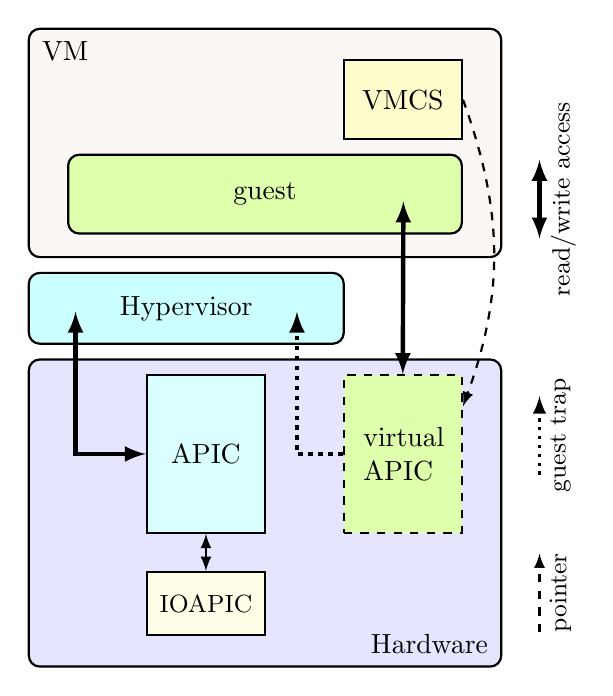
\begin{tikzpicture}

\node at (0,5) [rectangle, rounded corners, draw=black, thick, fill=Tan!10, minimum height = 2.9cm, minimum width = 6cm, anchor=south west] (vm) {};
\node [below right, inner sep=5pt] at (vm.north west) {VM};

\node at (0.5,5.3) [rectangle, rounded corners, draw=black, thick, fill=GreenYellow!40, minimum height = 1cm, minimum width = 5cm, anchor=south west] (g) {guest};
\node at (4.0,6.5) [rectangle, draw=black, thick, fill=yellow!20, minimum height = 1cm, minimum width = 1.5cm, anchor=south west] (vmcs) {VMCS};

\node at (0,3.9) [rectangle, rounded corners, draw=black, thick, fill=Cyan!20, minimum height = 0.9cm, minimum width = 4cm, anchor=south west] (hyper) {Hypervisor};

\node at (0,-0.2) [rectangle, rounded corners, draw=black, thick, fill=blue!10, minimum height = 3.9cm, minimum width = 6cm, anchor=south west] (hard) {};
\node [above left, inner sep=5pt] at (hard.south east) {Hardware};

\node at (1.5,1.5) [rectangle, draw=black, thick, fill=Cyan!15, minimum height = 2cm, minimum width = 1.5cm, anchor=south west] (apic) {APIC};
\node at (1.5,0.2) [rectangle, draw=black, thick, fill=yellow!10, minimum height = 0.8cm, minimum width = 1.5cm, anchor=south west] (ioapic) {\small{IOAPIC}};

\node at (4,1.5) [dashed, rectangle, draw=black, thick, fill=GreenYellow!40, minimum height = 2cm, minimum width = 1.5cm, anchor=south west, text width=1cm] (vapic) {virtual APIC};

\begin{scope}[>=latex]	
	\draw [ultra thick, <->] (apic.west) -| ([xshift=-40pt, yshift=12pt]hyper.south) ;
	\draw [ultra thick, <->] ([xshift=50pt, yshift=12pt]g.south) -- (vapic.north) ;
	\draw [ultra thick, dotted, ->] (vapic.west) -| ([xshift=40pt, yshift=12pt]hyper.south) ;
	\draw [thick, dashed, ->] (vmcs.east) to [bend left=20] ([yshift=4ex]vapic.east) ;
	\draw [thick, <->] (apic.south) -- (ioapic.north) ;

	\draw [ultra thick, <->] (6.5,5.25) -- (6.5,6.25) node [below, midway, rotate=90] {\small{read/write access}};
	\draw [very thick, dotted, ->] (6.5,2.25) -- (6.5,3.25) node [below, midway, rotate=90] {\small{guest trap}};
	\draw [thick, dashed, ->] (6.5,0.25) -- (6.5,1.25) node [below, midway, rotate=90] {\small{pointer}};
\end{scope}



\end{tikzpicture}
\end{center}
\ifreport
\caption{APIC Virtualization}
\fi
\label{fig-vapic}
\end{figure}
